%!TEX root = main.tex
\section{Introduction}
%Exploring multidiemnsional dataset is hard
\par Visual data exploration is the \emph{de facto} first step in understanding a multi-dimensional dataset. This exploration serves a variety of purposes: identifying trends and patterns, spotting outliers and anomalies, and verifying hypotheses. However, as datasets grow in size and complexity, visual data exploration ends up becoming challenging. For example, to identify patterns that merit further investigation, an analyst may need to explore different subsets of the data to determine when and where certain patterns occur. Generating and examining visualizations for this space of data subsets (which grows exponentially in number of attributes) is a major bottleneck in exploration.
%Drill-Down for exploration
\par One way of navigating this combinatorial space is to perform drill-downs on the lattice of data subsets. For example, a campaign manager who is interested in understanding the voting patterns across different demographics (say, race, gender, social class) using the 2016 US election exit polls~\cite{exitpolls} may first generate a bar chart for the entire population, where the x-axis shows the election candidates and the y-axis the percentage of votes for each of these candidates. In Figure~\ref{fig:elections_example}, the visualization at the top of the lattice corresponds to this overall population. They may then drill down to specific demographics of interest, say gender-based demographics, by generating bar charts for female voters (as shown in the second visualization at the second row of Figure 1).
\begin{figure}[ht!]
% 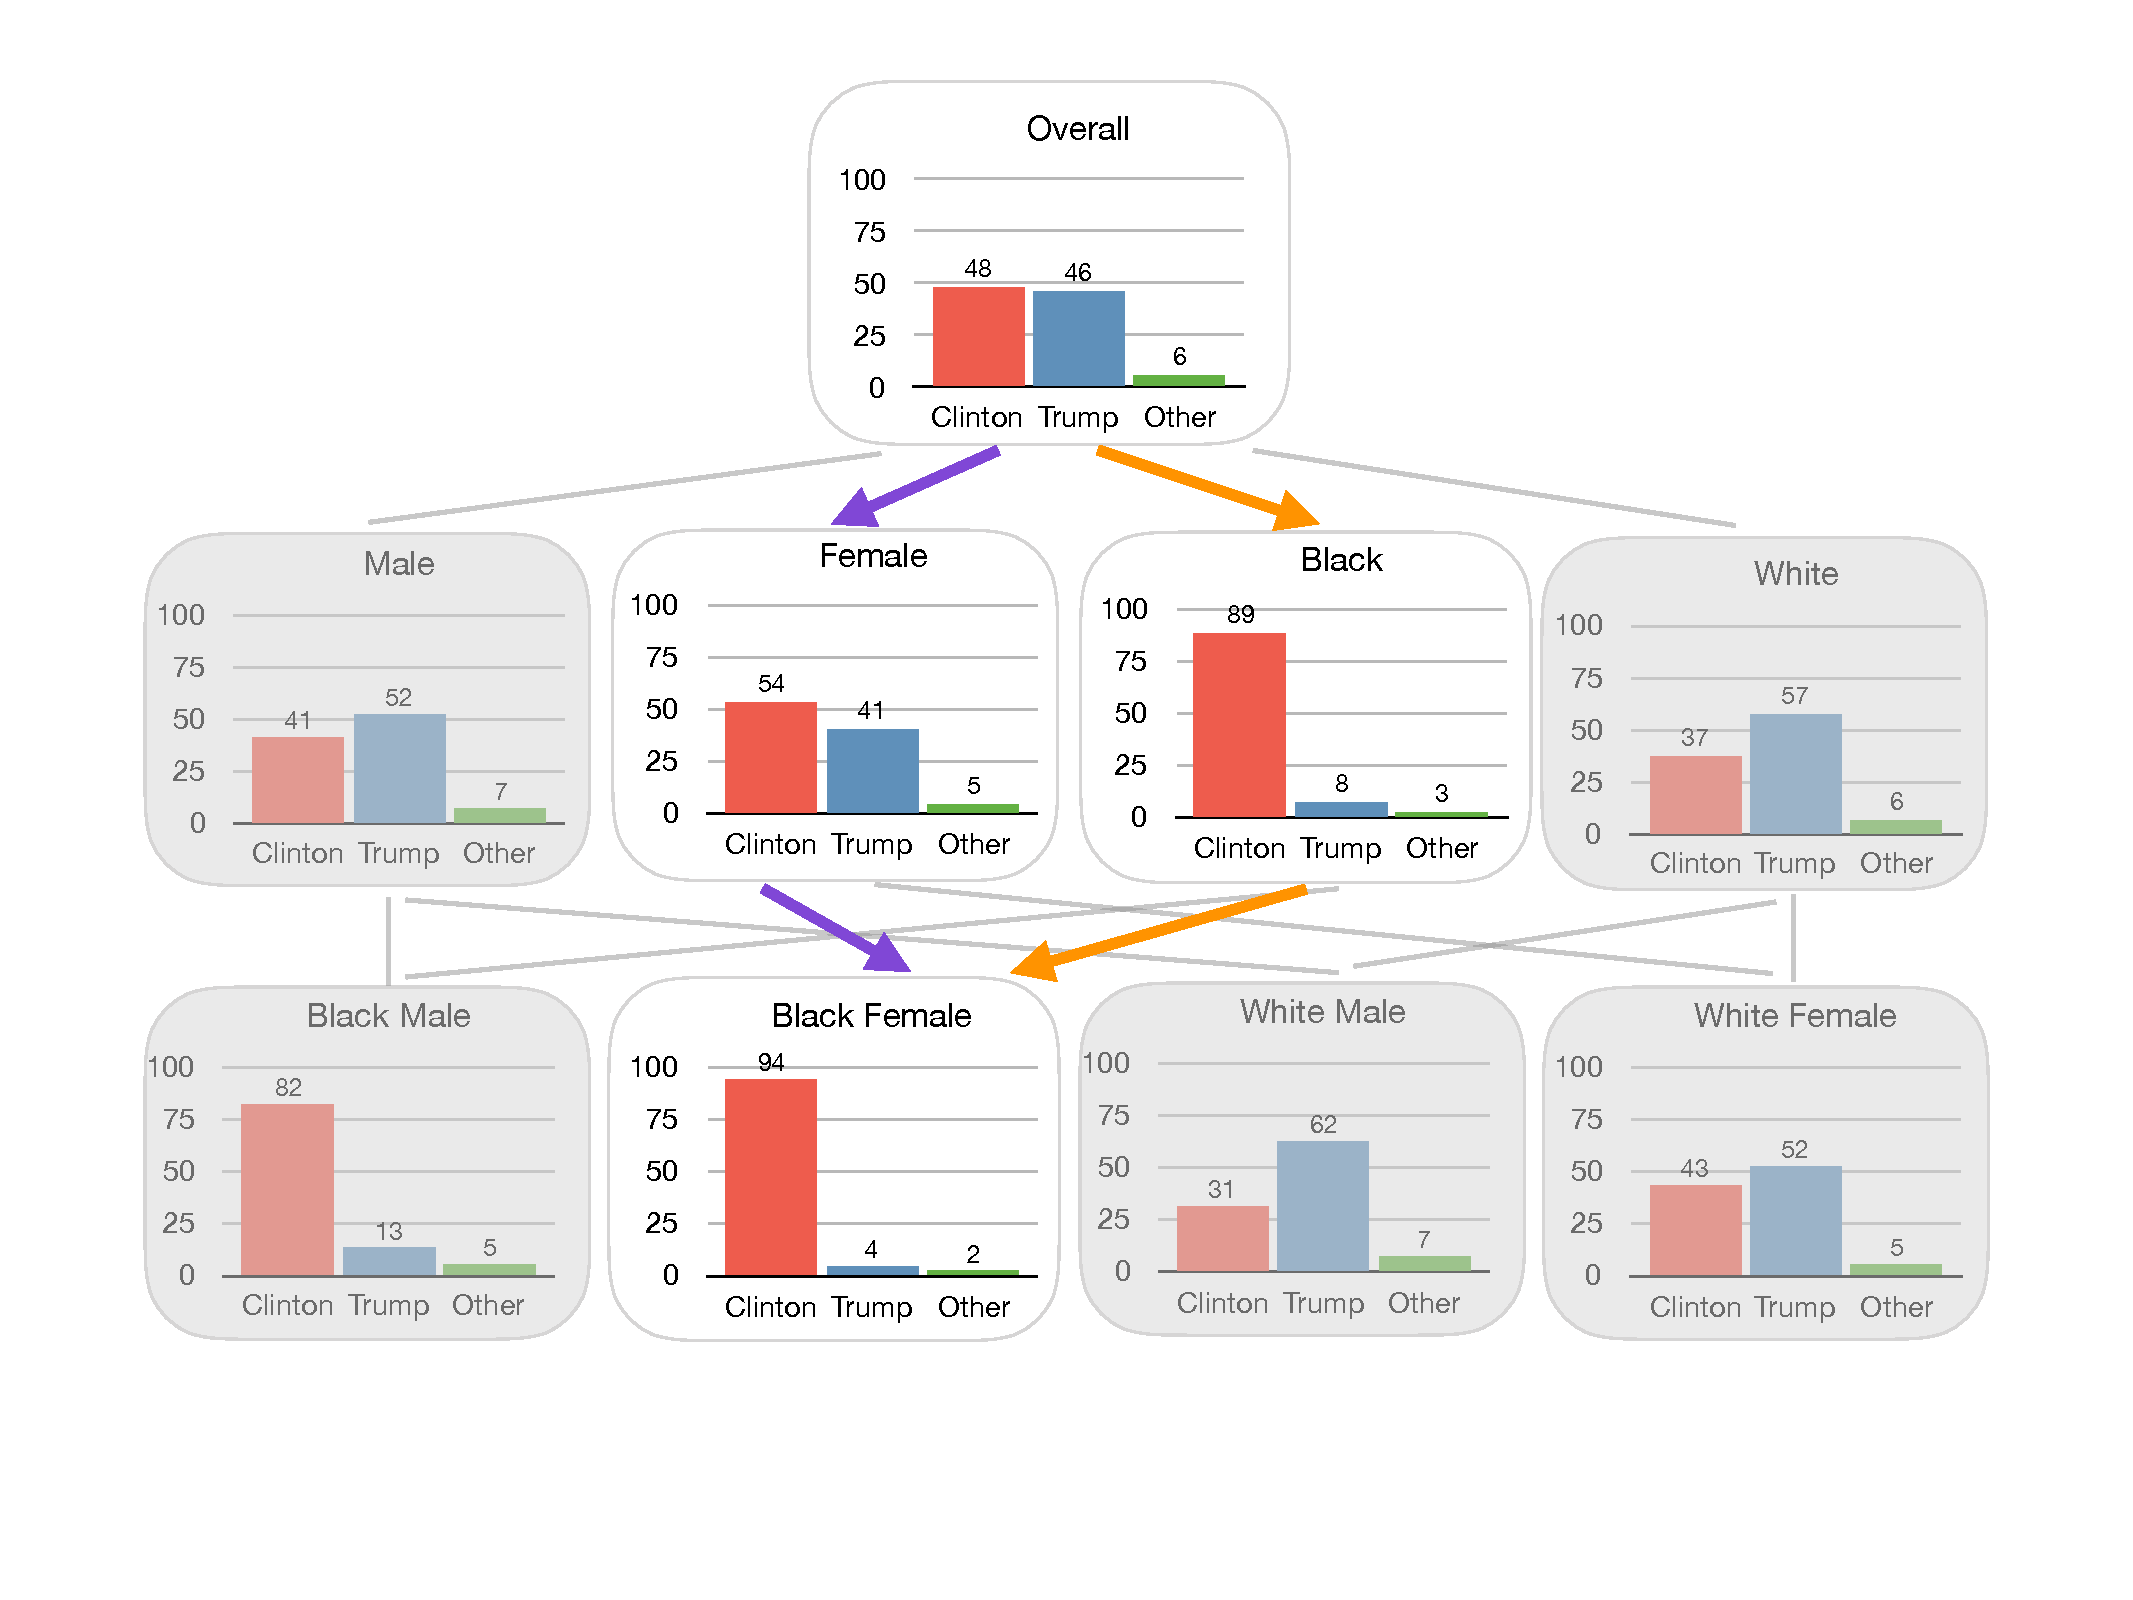
\includegraphics[width=\linewidth]{figures/elections_example_lattice.pdf}
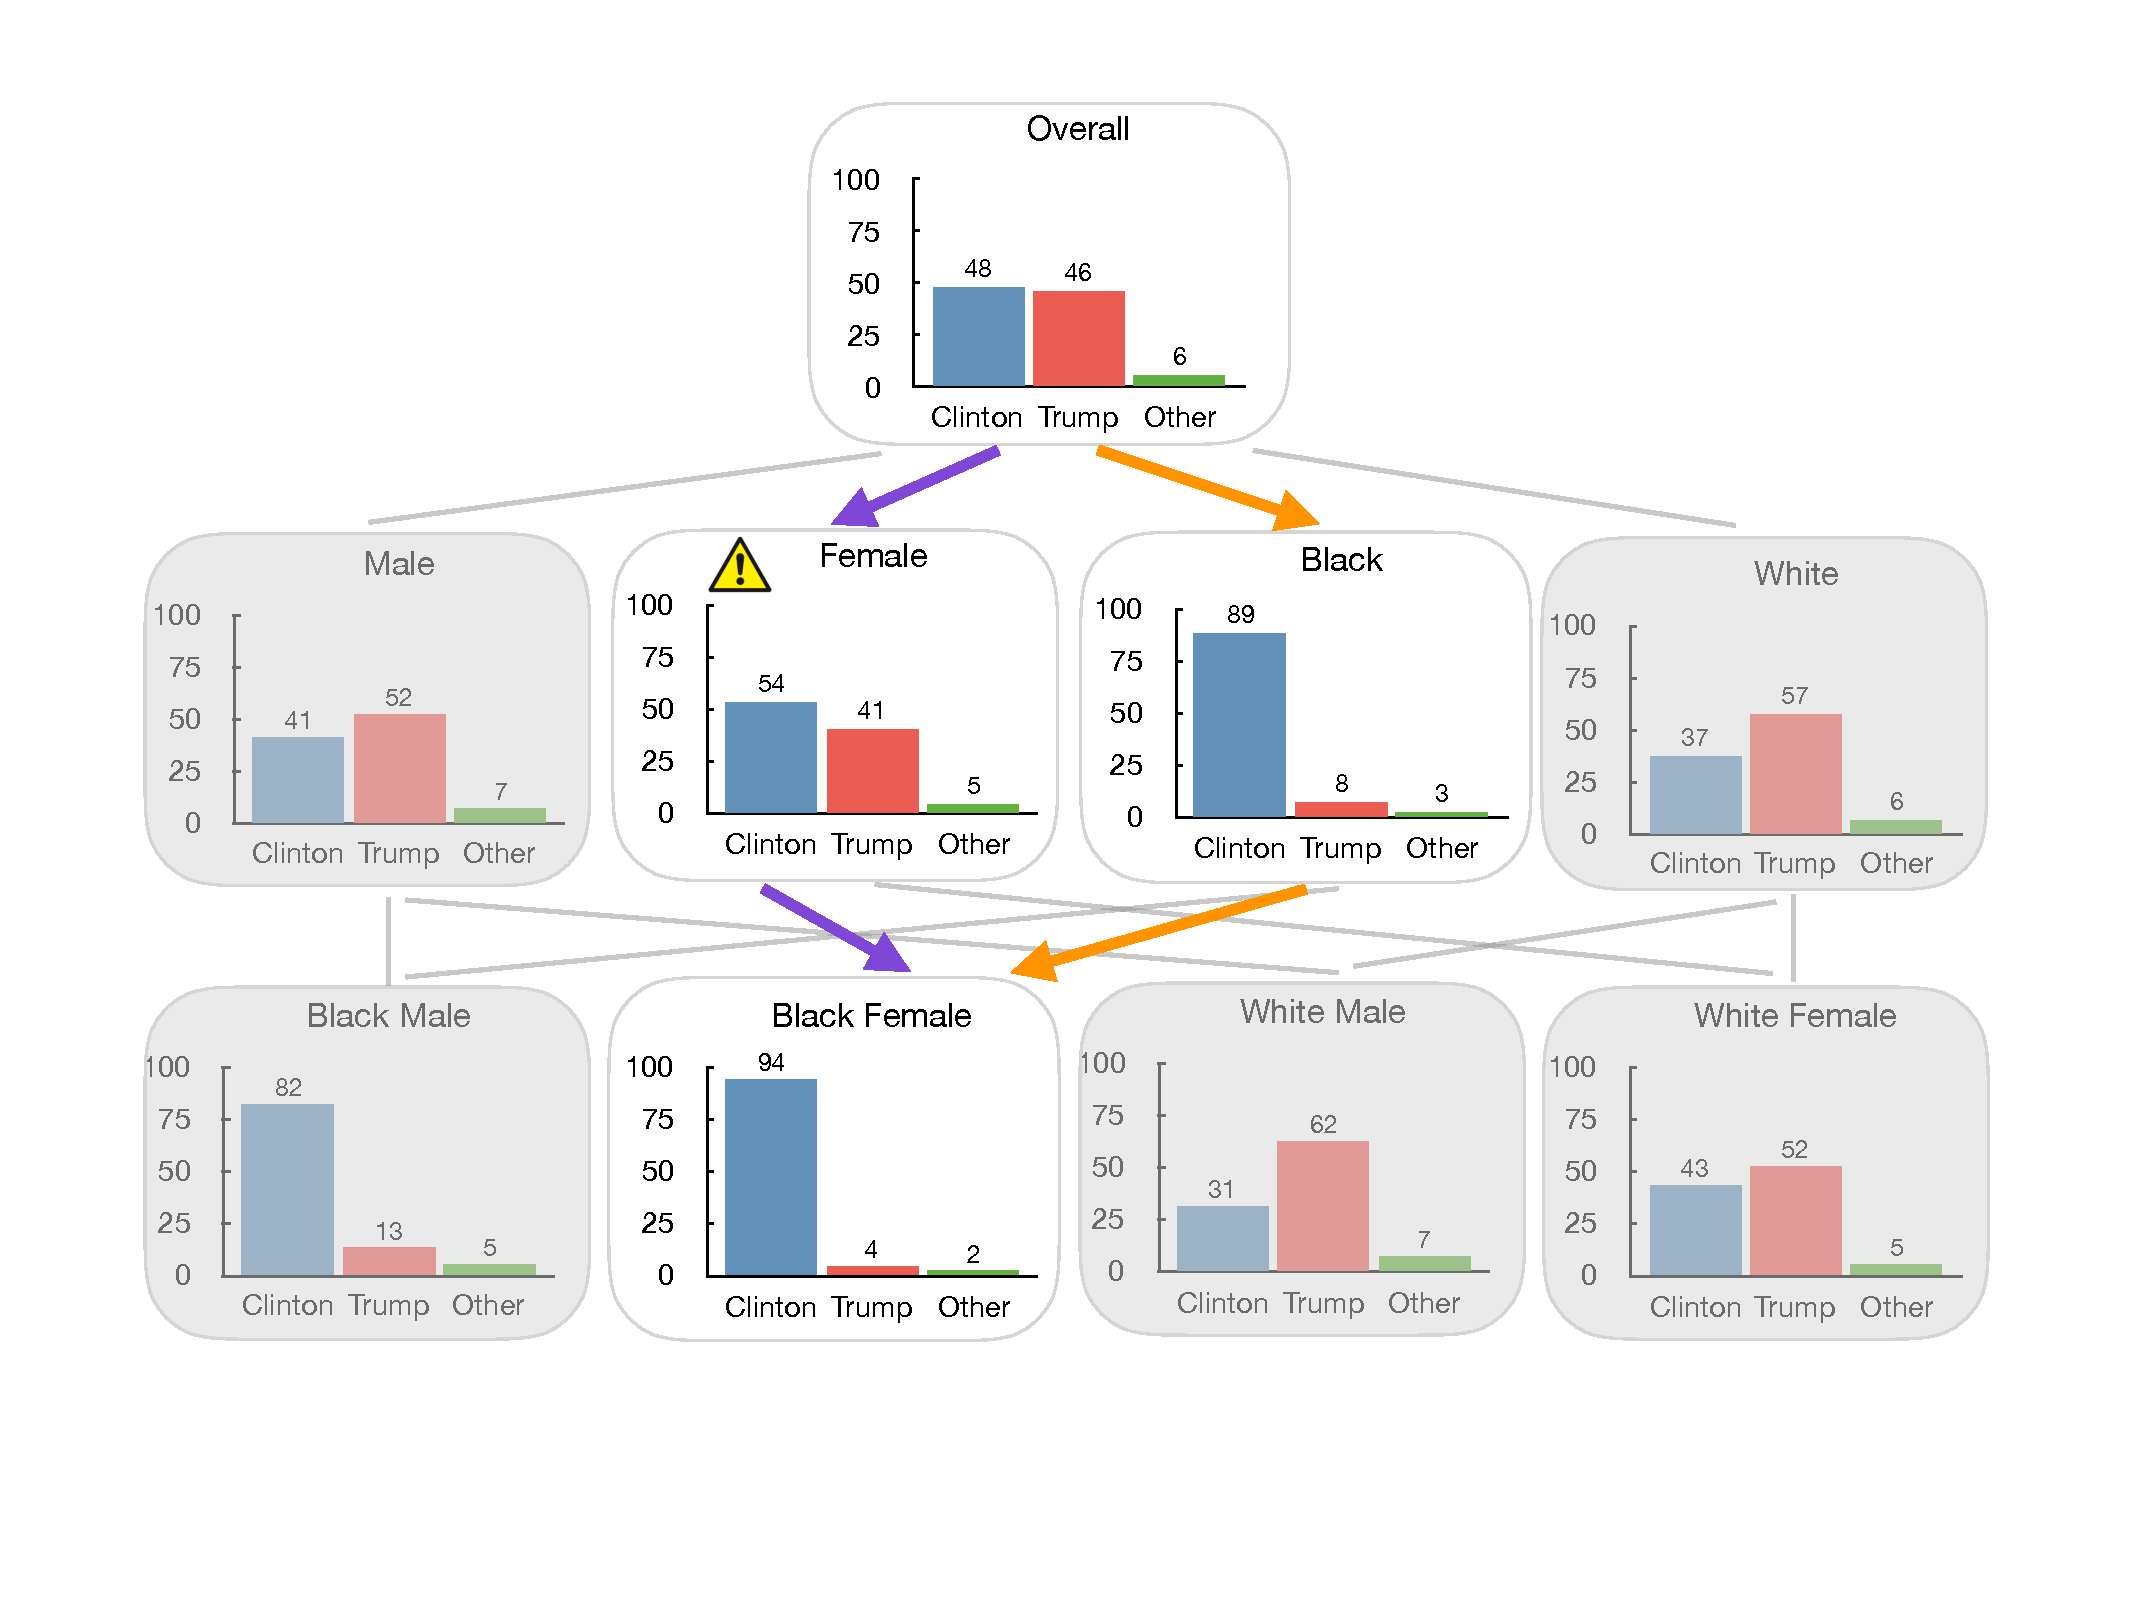
\includegraphics[width=\linewidth]{figures/elections_example_lattice_teaser.pdf}
\caption{Example data subset lattice illustrating the drill-down fallacy along the purple path as opposed to the informative orange path.}
\label{fig:elections_example}
\end{figure}
%Challenges associated with drill-down
\par There are three challenges associated with performing manual drill downs in this manner. First, it is often not clear which attributes to drill-down on. Analysts may use their intuition for this, but such arbitrary exploration may lead to large swaths of the lattice being ignored. Second, the path an analyst takes may lead to behavior that is not very surprising (insightful).  
For example, an analyst going from \texttt{Black} visualization to \texttt{Black Female} visualization in Figure 1 may find the two distributions to be similar, and therefore not surprising. This may well end up being wasted effort on the part of the analyst. Third, an analyst may encounter the \lq\lq drill-down fallacy\rq\rq : as shown in Figure~\ref{fig:elections_example}, an analyst can arrive at the \texttt{Black Female} visualization by going through the purple or orange drill-down path. An analyst who followed the purple path may be surprised at how drastically the \texttt{Black Female} voting behavior differs from that of \texttt{Female}. This behavior is no longer surprising if the analyst had gone down the orange path, where the proper reference (i.e., the vote distribution for \texttt{Black}) explains the vote distribution for \texttt{Black Female}. That is, even though the vote distribution for \texttt{Black Female} is very different from that of \texttt{Female}, it can be explained by a more general phenomenon or \lq\lq root cause\rq\rq ---the vote distribution for \texttt{Black} community. Attributing an overspecific cause to an effect, while ignoring the actual cause, not only leads to less interpretable explanations for the observed visualizations, but can also be detrimental to decision-making (in this case, it could lead to a misallocation of campaign funds).
\par The aforementioned example demonstrates the \emph{drill-down fallacy}---incomplete insights that result from potentially confounding factors not explored along a drill-down path. In particular, while performing a drill-down on a randomly selected path, an analyst may find a \lq\lq local difference\rq\rq\ in trends, without being aware of the more \lq\lq general phenomenon\rq\rq\ that could explain the trend of interest. In this case, they lack the proper parent reference (visualization) that explains the behavior of the visualization of interest. Thus, they are at risk of falling prey to the drill-down fallacy. A naive solution to avoid this fallacy is to explore all potential drill-down paths. Unfortunately, this approach does not scale with the increasing number of factors in the drill-down path.
\par In this paper, we present a visual data exploration tool that addresses the aforementioned challenges of exploration through three principles: (i) \textbf{Safety.} ensure that proper (informative) references are present to avoid the drill-down fallacy, (ii)  \textbf{Saliency.} identify interesting visualizations that convey new information (insights), and (iii) \textbf{Summarization.} succinctly convey the key insights. To facilitate safety, we develop a notion of \emph{informativeness}---the capability of a reference visualizations to explain the visualization of interest. To facilitate saliency, we characterize the notion of \emph{interestingness}---the difference between a visualization and its informative reference in terms of underlying data distribution. Finally, to facilitate summarization, we embrace \emph{collectiveness}---a connected network of visualizations that collectively offer informative insights. Based on these three principles, our tool, \system, automatically identifies a network of visualizations that succinctly conveys the key informative insights in a dataset. Our user study results demonstrate that our tool can guide an analyst towards meaningful insights for a variety of tasks. The contribution of this paper include:
\begin{denselist}
\item Introducing the novel concept of \emph{informativeness} that helps users identify meaningful insights that arise from something \textit{actually interesting} about the data (instead of confounding variables),
\item Designing a system that automatically identifies a network of visualizations that succinctly conveys the key informative insights in a dataset,
\item Demonstrating the efficacy of our system through a user study evaluation on how well users can retrieve interesting insights, judge the importance of attributes, and predict unseen visualizations against two other summarization baselines.
\end{denselist}